\documentclass{beamer}
\usetheme{Madrid}
\usepackage[utf8]{inputenc}
\usepackage[spanish]{babel}
\usepackage{amsmath}
\usepackage{graphicx} 

\title{Analizando el articulo: Uso de la programación lineal paramétrica en la solución de un problema de planeación de requerimiento de materiales bajo condiciones de incertidumbre }
\author{Lizbeth Estefany Caceres Tacora}
\date{}

\begin{document}

\frame{\titlepage}

% Frame 1: Introducción
\begin{frame}{Introducción}
\begin{itemize}
    \item El artículo aborda un problema de Planeación de Requerimiento de Materiales (MRP) en la industria automotriz bajo condiciones de incertidumbre.
    \item El articulo tiene como idea principal la toma de decisiones de incertidumbre, usando modelos matemáticos como la programación lineal junto con la teoria de conjuntos difusos.
    \item El objetivo es mostrar como se puede aplicar la programacion lineal para resolver problemas reales en la industria, incluso cuando la informacion no es precisa.
\end{itemize}
\end{frame}

% Frame 2: Aplicacion de la programacion lineal
\begin{frame}{Aplicacion de la programacion lineal}
\begin{itemize}
    \item Para la función objetivo, se partió desde la teoría de programación determinista y difusa, donde se emplean la función de pertenencia y la función de pretenencia para las restricciones, dando como resultado:
    \centering
    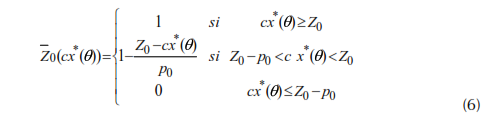
\includegraphics[width=0.6 \linewidth]{pl_1.png}
    \item En el artículo, el modelo 6 se aplica para determinar el costo de producción del ensamble de la puerta izquierda de un automóvil.
    \centering
    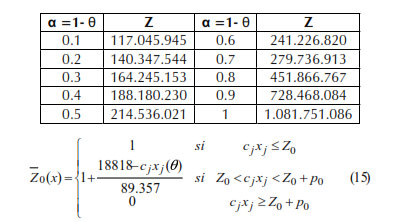
\includegraphics[width=0.65\linewidth]{pl_2.png}
    
    \end{itemize}
\end{frame}

% Frame 3: Modelo Matemático Difuso
\begin{frame}{Aaplicacion de la programacion lineal}
\begin{itemize}
    \item Se calcula el índice de compatibilidad de cada solución con los niveles de aspiración del decisor.
    
    \centering
    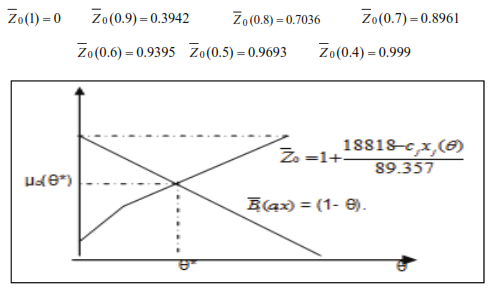
\includegraphics[width=0.65\linewidth]{pl_3.png}
    
    \item Para encontrar la solución óptima correspondiente, debe elegirse $\theta^*$ tal que:
\[
\mu_D(\theta^*) = \max_{\theta} \mu_D(\theta) = \max_{\theta} \left( \min \left( Z_0(\theta), B_c(\theta) \right) \right)
\]
    \item Donde Z = 28098.990; Nivel de satisfacción = 0.6272 
\end{itemize}
\end{frame}

% Frame 4: Aplicación y Resultados
\begin{frame}{Aplicación y Resultados}
\begin{itemize}
    \item El costo en el que se incurre en la solución obtenida con
esta metodología es alto, al considerar la capacidad y la demanda como valores inciertos, los costos pueden ser aún mucho mayores, por lo que el costo del plan Z = 28098.990 es una solución intermedia que equilibra los criterios pesimistas y optimistas.

    \centering
    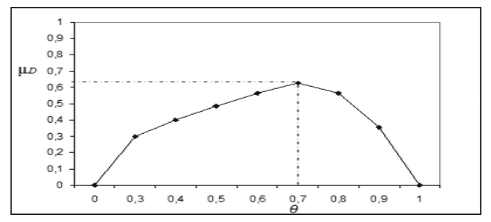
\includegraphics[width=0.65\linewidth]{pl_4.png}
    
\end{itemize}
\end{frame}

% Frame 5: Conclusiones
\begin{frame}{Conclusiones}
\begin{itemize}
    \item La programación lineal paramétrica difusa es eficaz para enfrentar problemas de planificación con datos imprecisos.
    \item Permite generar soluciones flexibles y realistas en entornos industriales.
    \item Se destaca la importancia de considerar la incertidumbre desde la formulación matemática.
    \item Aporta valor en la toma de decisiones operativas y estratégicas en sistemas productivos complejos.
\end{itemize}
\end{frame}

\end{document}
